\documentclass[11pt,paper={letter}]{scrartcl}
\usepackage{jrdobaob}



\begin{document}

\title{MATHWIZZ 2023 Elims Problems (Part 1)}
\author{{\sffamily \textbf{Problems of the Week}} (2023 Edition)}
\maketitle

\setlength{\unitlength}{1in}
\begin{picture}(2,0)
\put(0.7,1.3){\hbox{
\includegraphics[width = 5in]{logo.png}}}
\end{picture}

After many months of hiatus, I have finally exploit the opportunity to begin another edition of my \textbf{Problems of the Week} edition for this year! The following problems are from the recent \textbf{MATHWIZZ 2023 Elimination Round}. THe first ten problems of the round are presented here with my solutions while the second and last ten questions will be on next week. If you see any typographical errors, wrong calculations, feel free to contact me at \mailto{jrdobaob@addu.edu.ph}

\

\textbf{Note.} Some of the problems are rephrased either for fun or for saving time on typing these stuff.


\begin{enumerate}[label=\textbf{\arabic*}.]
\item Jim spent $\frac{1}{4}$ of his starting pocket money on food and 50 pesos on school supplies. As a result, he has $\frac{5}{12}$ of his starting pocket money remaining. By how much did Jim spend on food alone?

\ans{$\PHP$ 37.5}

\sol Let $x$ be Jim's pocket money. So, $$x - \dfrac{1}{4}x - 50 = \dfrac{5}{12}x \Longleftrightarrow \dfrac{3x}{4} - \dfrac{5x}{12}  = 50 \Longleftrightarrow \dfrac{x}{3} = 50.$$ We see that Jim's money is 150 pesos. Therefore, Jim spent \fbox{$150/4 =  \PHP 37.5$} on his food alone.

\item Find all values of $x$, $0\dg \leq x\dg < 360\dg$, such that $\sin x = \sin 2x.$

\ans{60, 300}

\sol By double-angle identity, $\sin 2x = 2\sin x \cos x$. Hence, 

\begin{equation*}
    \begin{array}{rcl}
         \sin x & = & \sin2x \\
     \sin x    & = & 2\sin x \cos x  \\
     1    & = & 2\cos x  \\
     \frac{1}{2}    & = & \cos x  \\
         
    \end{array}
\end{equation*}

We see that the possible values of $x$ are \fbox{$60$ and $300$}. 
\item Paula and Pilar have money with ratio $1:9$ respectively. After Pilar gave Paula 450 pesos, the ratio is $3:2$. How much money did Pilar have from the beginning?

\ans{$\PHP 810$}

\sol Mathematically, that is just

\begin{equation*}
    \dfrac{a + 450}{9a - 450} = \dfrac{3a}{2a} \Longleftrightarrow 2250 = 25a \Longleftrightarrow a = 90
\end{equation*}

Therefore, Pilar have $9 \times 90 = \fbox{\PHP 810}$ pesos at the beginning
\item If 2.4 wids $=$ 4.2 wads, and 1.6 wids $=$ 3.5 wods, how many wads are there in 10 wods?

\ans{$64/7$ wads}

\sol We see that 1.0 wad is equivalent to 0.5 wid, and $ \frac{16}{35} \ \text{wid} = 1 \ \text{wod}$. Therefore, $$ \implies 10 \ \text{wods} \times \frac{\frac{16}{35} \ \text{wid}}{1 \ \text{wod}} \times \frac{2 \ \text{wads}}{1 \ \text{wid}} =\boxed{64/7 \ \text{wads}} $$

\item Determine the value of $\displaystyle{{\int_0}^2 (x-2)^5(x+1) \ dx}$.

\ans{$-96/7$}

\sol Let $u = x-2$ and $du = dx$. Therefore,

\begin{equation*}
    \begin{array}{rcl}
        \displaystyle{{\int_0}^2 (x-2)^5(x+1) \ dx} & = & \displaystyle{{\int_0}^2 u^5(u+3) \ du} \\

& &\\ 

          & = & \displaystyle{{\int_0}^2 u^6 + 3u^5 \ du} \\

          && \\

          & = & \dfrac{u^7}{7} + \dfrac{u^6}{2} \ {\color{red} \bigg |_{0}^2} \\

           && \\

          & = & \dfrac{(x-2)^7}{7} + \dfrac{(x-2)^6}{2} \ {\color{red} \bigg |_{0}^2} \\

          && \\

          & = & \left(\dfrac{({\color{red} 2}-2)^7}{7} + \dfrac{({\color{red} 2}-2)^6}{2} \right) - \left(\dfrac{({\color{red} 0}-2)^7}{7} + \dfrac{({\color{red} 0}-2)^6}{2} \right)  \\

          && \\

          & = & \dfrac{128}{7} - 32 \\

          && \\

          & = & \boxed{-96/7} \\
    \end{array}
\end{equation*}

\item How many whole numbers from 1 to 1,000 are divisible by 4, but not divisible by 3?

\ans{167}

\sol Let $N$ be the number of whole integers that are divisible by 4 but not by 3. By the principle of exclusion-inclusion, this is just 

\begin{equation*}
    \begin{array}{rcl}

    N &=& P(3|N) - P(12|N)\\
        N & = & \bigg \lfloor \dfrac{1000}{4} \bigg \rfloor - \bigg \lfloor \dfrac{1000}{12} \bigg \rfloor   \\

        &=& 167 \\
         
    \end{array}
\end{equation*}

\item Compute: $i^{1^2} + i^{2^2} + \ldots +i^{2022^2}+ i^{2023^2}$. ($i = \sqrt{-1}$)

\ans{$1011 + 1012i$}

\sol Recall the following properties:

\begin{itemize}
    \item $i = \sqrt{-1}$
    \item $i^2 = {-1}$
    \item $i^3 = -i$
    \item $i^4 = 1$
\end{itemize}

This gives us the motivation to use the modulo 4 in each exponent of each term. Notice that an exponent $(2k+1)^2  \equiv 4k^2 + 4k + 1 \equiv 1\pmod{4}$ and an odd exponent $(2k)^2 \equiv 0 \pmod{4}.$ Therefore, our answer is $1011(i^0) + 1012(i^1) = \boxed{1011 + 1012i.}$
\item Point $P$ is outside a rectangle $ABCD$ such that $PA = 6, PB = 11$ and $PC = 13$. Find $PD$.

\ans{$2\sqrt{21}$}


\sol {\sffamily (Inspired from the solution of Benedict Rodil).} The figure can be configured like this:

\begin{center}
    



\tikzset{every picture/.style={line width=0.75pt}} %set default line width to 0.75pt        

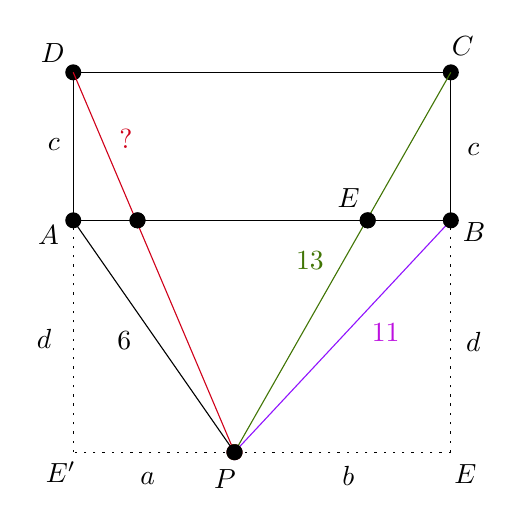
\begin{tikzpicture}[x=0.75pt,y=0.75pt,yscale=-1,xscale=1]
%uncomment if require: \path (0,705); %set diagram left start at 0, and has height of 705

%Straight Lines [id:da5229409525016646] 
\draw [color={rgb, 255:red, 144; green, 19; blue, 254 }  ,draw opacity=1 ]   (380.72,256.74) -- (276.49,368.44) ;
\draw [shift={(276.49,368.44)}, rotate = 133.02] [color={rgb, 255:red, 144; green, 19; blue, 254 }  ,draw opacity=1 ][fill={rgb, 255:red, 144; green, 19; blue, 254 }  ,fill opacity=1 ][line width=0.75]      (0, 0) circle [x radius= 3.35, y radius= 3.35]   ;
%Straight Lines [id:da6207630317501531] 
\draw    (198.8,185.44) -- (380.72,185.44) ;
\draw [shift={(380.72,185.44)}, rotate = 0] [color={rgb, 255:red, 0; green, 0; blue, 0 }  ][fill={rgb, 255:red, 0; green, 0; blue, 0 }  ][line width=0.75]      (0, 0) circle [x radius= 3.35, y radius= 3.35]   ;
\draw [shift={(198.8,185.44)}, rotate = 0] [color={rgb, 255:red, 0; green, 0; blue, 0 }  ][fill={rgb, 255:red, 0; green, 0; blue, 0 }  ][line width=0.75]      (0, 0) circle [x radius= 3.35, y radius= 3.35]   ;
%Straight Lines [id:da7602442963438456] 
\draw    (380.72,185.44) -- (380.72,256.74) ;
%Straight Lines [id:da6218057684326268] 
\draw    (198.8,185.44) -- (198.8,256.74) ;
%Straight Lines [id:da41896731966254896] 
\draw [color={rgb, 255:red, 208; green, 2; blue, 27 }  ,draw opacity=1 ]   (198.8,185.44) -- (276.49,368.44) ;
\draw [shift={(276.49,368.44)}, rotate = 67] [color={rgb, 255:red, 208; green, 2; blue, 27 }  ,draw opacity=1 ][fill={rgb, 255:red, 208; green, 2; blue, 27 }  ,fill opacity=1 ][line width=0.75]      (0, 0) circle [x radius= 3.35, y radius= 3.35]   ;
%Straight Lines [id:da40295221798909786] 
\draw [color={rgb, 255:red, 65; green, 117; blue, 5 }  ,draw opacity=1 ]   (380.72,185.44) -- (276.49,368.44) ;
\draw [shift={(276.49,368.44)}, rotate = 119.66] [color={rgb, 255:red, 65; green, 117; blue, 5 }  ,draw opacity=1 ][fill={rgb, 255:red, 65; green, 117; blue, 5 }  ,fill opacity=1 ][line width=0.75]      (0, 0) circle [x radius= 3.35, y radius= 3.35]   ;
%Straight Lines [id:da08302845807052806] 
\draw [color={rgb, 255:red, 0; green, 0; blue, 0 }  ,draw opacity=1 ]   (198.8,256.74) -- (276.49,368.44) ;
\draw [shift={(276.49,368.44)}, rotate = 55.18] [color={rgb, 255:red, 0; green, 0; blue, 0 }  ,draw opacity=1 ][fill={rgb, 255:red, 0; green, 0; blue, 0 }  ,fill opacity=1 ][line width=0.75]      (0, 0) circle [x radius= 3.35, y radius= 3.35]   ;
%Straight Lines [id:da5866409496678218] 
\draw    (198.8,256.74) -- (229.75,256.74) ;
\draw [shift={(229.75,256.74)}, rotate = 0] [color={rgb, 255:red, 0; green, 0; blue, 0 }  ][fill={rgb, 255:red, 0; green, 0; blue, 0 }  ][line width=0.75]      (0, 0) circle [x radius= 3.35, y radius= 3.35]   ;
\draw [shift={(198.8,256.74)}, rotate = 0] [color={rgb, 255:red, 0; green, 0; blue, 0 }  ][fill={rgb, 255:red, 0; green, 0; blue, 0 }  ][line width=0.75]      (0, 0) circle [x radius= 3.35, y radius= 3.35]   ;
%Straight Lines [id:da8864597638356757] 
\draw    (229.75,256.74) -- (340.66,256.74) ;
\draw [shift={(340.66,256.74)}, rotate = 0] [color={rgb, 255:red, 0; green, 0; blue, 0 }  ][fill={rgb, 255:red, 0; green, 0; blue, 0 }  ][line width=0.75]      (0, 0) circle [x radius= 3.35, y radius= 3.35]   ;
\draw [shift={(229.75,256.74)}, rotate = 0] [color={rgb, 255:red, 0; green, 0; blue, 0 }  ][fill={rgb, 255:red, 0; green, 0; blue, 0 }  ][line width=0.75]      (0, 0) circle [x radius= 3.35, y radius= 3.35]   ;
%Straight Lines [id:da9529914212744153] 
\draw    (340.66,256.74) -- (380.72,256.74) ;
\draw [shift={(380.72,256.74)}, rotate = 0] [color={rgb, 255:red, 0; green, 0; blue, 0 }  ][fill={rgb, 255:red, 0; green, 0; blue, 0 }  ][line width=0.75]      (0, 0) circle [x radius= 3.35, y radius= 3.35]   ;
\draw [shift={(340.66,256.74)}, rotate = 0] [color={rgb, 255:red, 0; green, 0; blue, 0 }  ][fill={rgb, 255:red, 0; green, 0; blue, 0 }  ][line width=0.75]      (0, 0) circle [x radius= 3.35, y radius= 3.35]   ;
%Straight Lines [id:da974821710698393] 
\draw  [dash pattern={on 0.84pt off 2.51pt}]  (198.8,368.44) -- (198.8,256.74) ;
%Straight Lines [id:da5443493207245891] 
\draw  [dash pattern={on 0.84pt off 2.51pt}]  (276.49,368.44) -- (198.8,368.44) ;
%Straight Lines [id:da9905285492985312] 
\draw  [dash pattern={on 0.84pt off 2.51pt}]  (380.72,368.44) -- (380.72,256.74) ;
%Straight Lines [id:da6760403733321232] 
\draw  [dash pattern={on 0.84pt off 2.51pt}]  (380.72,368.44) -- (276.49,368.44) ;

% Text Node
\draw (271.91,381.27) node    {$P$};
% Text Node
\draw (186.83,264.03) node    {$A$};
% Text Node
\draw (391.9,262.44) node    {$B$};
% Text Node
\draw (188.86,176.09) node    {$D$};
% Text Node
\draw (386.47,172.92) node    {$C$};
% Text Node
\draw (224.14,217.29) node  [color={rgb, 255:red, 208; green, 2; blue, 27 }  ,opacity=1 ]  {$?$};
% Text Node
\draw (312.87,275.91) node  [color={rgb, 255:red, 65; green, 117; blue, 5 }  ,opacity=1 ]  {$13$};
% Text Node
\draw (349.31,310.77) node  [color={rgb, 255:red, 189; green, 16; blue, 224 }  ,opacity=1 ]  {$11$};
% Text Node
\draw (223.35,314.73) node  [color={rgb, 255:red, 0; green, 0; blue, 0 }  ,opacity=1 ]  {$6$};
% Text Node
\draw (331.46,245.81) node    {$E$};
% Text Node
\draw (192.82,378.1) node    {$E'$};
% Text Node
\draw (387.71,378.9) node    {$E$};
% Text Node
\draw (234.67,381.27) node    {$a$};
% Text Node
\draw (331.32,379.69) node    {$b$};
% Text Node
\draw (184.76,313.94) node    {$d$};
% Text Node
\draw (391.53,315.52) node    {$d$};
% Text Node
\draw (391.53,222.83) node    {$c$};
% Text Node
\draw (189.52,220.45) node    {$c$};


\end{tikzpicture}


\end{center}

Invoking the Pythagorean theorem, we have the following system of quadratic equations

\begin{equation*}
    \begin{cases}
    d^2 +a^2 = 36 \\ d^2 + b^2 = 121 \\ (c+d)^2 + b^2 = 169 \\ (c+d)^2 + a^2 = PD^2
    \end{cases}
\end{equation*}

Subtract the second equation from the first and you get $a^2 - b^2 = -85$. Add this equation to the third equation and you get $$[(c+d)^2 + b^2] + [a^2 - b^2] = PD^2 \Longleftrightarrow 169 + (-85) = 84 = PD^2.$$ Therefore, \fbox{$PD = 2\sqrt{21}$}. 


\item Denote $f(x)$ as a polynomial function whereas $f(2x-1) = 8x^2 -10x +7$. Find the remainder of $f(x)$ divided by $(x-3).$

\ans{$19$}

\sol Let $u = x$: $$f(2a -1) = 8a^2 - 10a + 7.$$ Next, let $x = 2a - 1 \Longleftrightarrow a = \frac{x+1}{2}$:

\begin{equation*}
    \begin{array}{rcl}
         f\left(2\left(\dfrac{x+1}{2}\right) - 1\right)&  = & 8\left(\dfrac{x+1}{2}\right)^2 - 10\left(\dfrac{x+1}{2}\right) + 7\\

         &=& \\

           f(x)&  = & 2\left(x^2 + 2x +1\right) - 5(x+1) + 7\\

           &  = & 2x^2 + 4x + 2 -5x - 5 + 7\\

           & = & 2x^2 - x + 4 \\
    \end{array}
\end{equation*}

Now rewriting $f(x)$ in terms of $x-3$ gives us $$f(x) =
2(x-3)^2 + 11x - 14 \Longleftrightarrow [2(x-3)^2 ]+ [11(x-3) + 19] $$ Therefore, the remainder of $f(x)$ is \fbox{$19.$}

\item Determine the value of $\left(1 - \dfrac{1}{2^2}\right)\left(1 - \dfrac{1}{3^2}\right)\left(1 - \dfrac{1}{4^2}\right)\ldots\left(1 - \dfrac{1}{2022^2}\right)\left(1 - \dfrac{1}{2023^2}\right)$

\ans{$1012/2023$}

\soln1 Evaluate every term and we have:

\begin{equation*}
    \begin{array}{rcl}
         N &  = & \left(\dfrac{(1)(3)}{2^2}\right)\left(\dfrac{(2)(4)}{3^2}\right)\left(\dfrac{(3)(5)}{4^2}\right)\ldots\left(\dfrac{(2021)(2023)}{2022^2}\right)\left(\dfrac{(2022)(2024)}{2023^2}\right)\\

         & = & \\

         & = & \dfrac{1 \times 2 \times 3^2 \times 4^2 \times 5^2 \times \ldots \times 2023 \times 2024 }{(2\times 3 \times 4 \times \ldots \times 2022 \times 2023)^2}
    \end{array}
\end{equation*}

This is similar to the expression: $\dfrac{(1 \times 2 \times 3 \times \ldots \times 2022)(1 \times 2 \times 3 \times \ldots 2023 \times 2024)}{(1\times 2\times 3 \times \ldots \times 2022 \times 2023)^2} = \dfrac{2022! 2024!}{(2023!)^2}$

So, $N$ is just 

\begin{equation*}
    \begin{array}{rcl}

         N & = & \dfrac{\dfrac{2022!2024!}{2023!2023!}}{2}\\

         && \\

          N & = & \dfrac{2024}{2(2023)}\\

          & = & \boxed{\dfrac{1012}{2023}}\\
    \end{array}
\end{equation*}

\soln2 The expression can be rewritten as $$\left[\left(\dfrac{3}{2}\right)\left(\dfrac{4}{3}\right)\ldots\left(\dfrac{2023}{2022}\right)\left(\dfrac{2024}{2023}\right)\right] \ldots \left[\left(\dfrac{1}{2}\right)\left(\dfrac{2}{3}\right)\ldots\left(\dfrac{2021}{2022}\right)\left(\dfrac{2022}{2023}\right)\right]$$ which is equal to $$\dfrac{2024!}{2(2023!)} \times \dfrac{2022!}{2023!} = \boxed{\dfrac{1012}{2023}}$$


\end{enumerate}

\emph{Special thanks to Engr. Isaiah James Maling for posting the problems of the contest in his \href{https://www.facebook.com/photo/?fbid=193779303389619&set=pb.100082726513011.-2207520000.}{Facebook page}!} \footnote{Link to the problems: \url{https://www.facebook.com/photo/?fbid=193779303389619&set=pb.100082726513011.-2207520000.}}
\end{document}
